\documentclass[11pt,letterpaper]{article}
\usepackage[lmargin=1in,rmargin=1in,tmargin=1in,bmargin=1in]{geometry}
\usepackage{../style/homework}
\usepackage{../style/commands}
\setbool{quotetype}{true} % True: Side; False: Under
\setbool{hideans}{true} % Student: True; Instructor: False

% -------------------
% Content
% -------------------
\begin{document}

\homework{6: Due 01/12}{I'm always thinking one step ahead, like a carpenter that makes stairs.}{Andy Bernard, The Office}

% Problem 1
\problem{10} A linear function is plotted below. Find the equation of this linear function. 
	\[
	\fbox{
	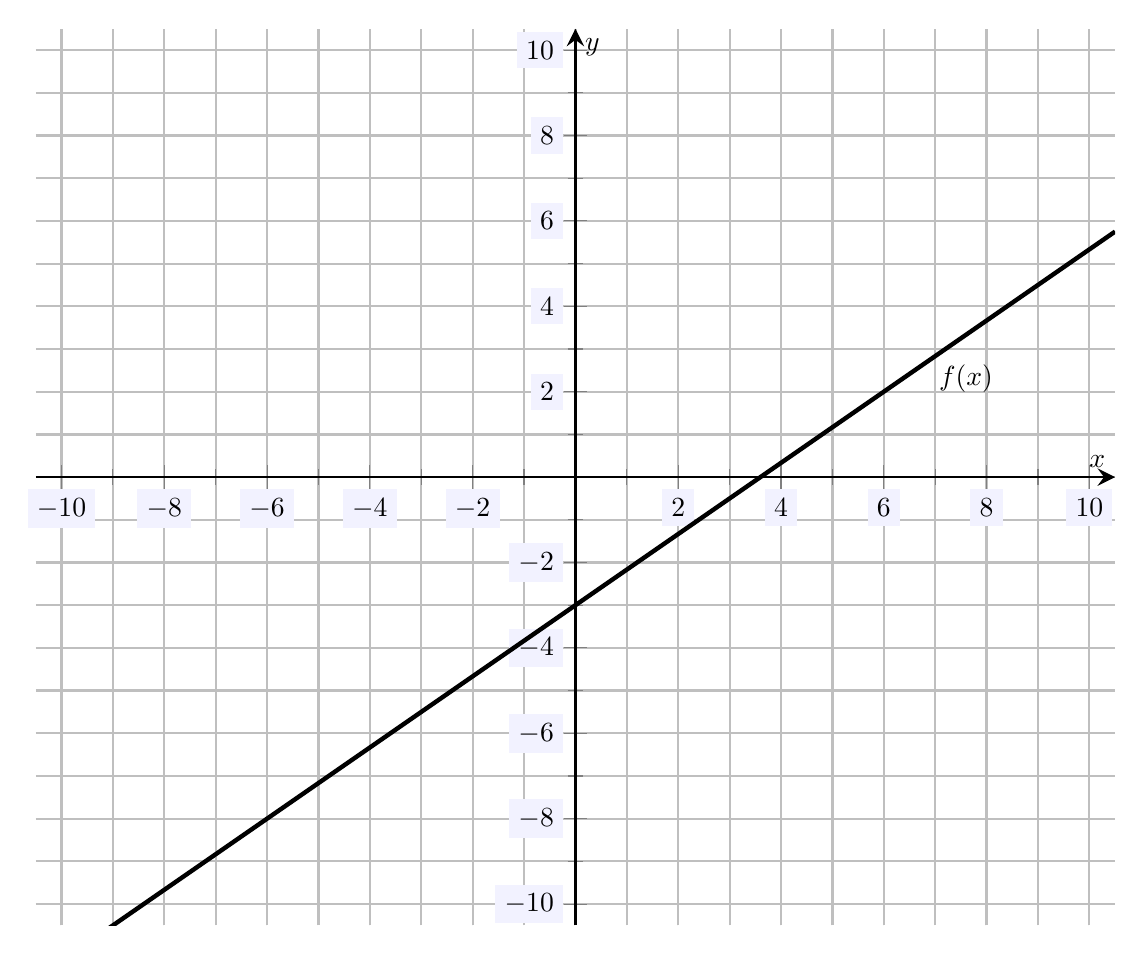
\begin{tikzpicture}[scale=2,every node/.style={scale=0.5}]
	\begin{axis}[
	grid=both,
	axis lines=middle,
	ticklabel style={fill=blue!5!white},
	xmin= -10.5, xmax=10.5,
	ymin= -10.5, ymax=10.5,
	xtick={-10,-8,-6,-4,-2,0,2,4,6,8,10},
	ytick={-10,-8,-6,-4,-2,0,2,4,6,8,10},
	minor tick = {-10,-9,...,10},
	xlabel=\(x\),ylabel=\(y\),
	]
	\node at (7.6,2.3) {$f(x)$};
	\addplot[thick, domain= -10.5:10.5] ({x},{5/6*x - 3});
	\end{axis}
	\end{tikzpicture}
	}
	\]



\newpage



% Problem 2
\problem{10} Determine if the following pairs of lines are the same, perpendicular, parallel, or none of these. 
	\[
	\begin{aligned}
	\ell_1&: & y= \frac{3}{2}\,&x + 9 \\
	\ell_2&: & 9x - 6y&= 12
	\end{aligned}
	\]



\newpage



% Problem 3
\problem{10} Determine if the following pairs of lines are the same, perpendicular, parallel, or none of these. 
	\[
	\begin{aligned}
	\ell_1&: & 2x - 3y&= 5 \\
	\ell_2&: & 6x + 5y&= -3
	\end{aligned}
	\]



\newpage



% Problem 4
\problem{10} Determine if the following pairs of lines are the same, perpendicular, parallel, or none of these. 
	\[
	\begin{aligned}
	\ell_1&: & y= -2x& + 7 \\
	\ell_2&: & -3x + 6y&= 15
	\end{aligned}
	\]



\newpage



% Problem 5
\problem{10} Find the equation of the line passing through the points $(6, 21)$ and $(-9, -19)$. \pspace



\newpage



% Problem 6
\problem{10} Find the equation of the line perpendicular to $y= 4 - 5x$ that passes through the point $(3, -1)$. \pspace



\newpage



% Problem 7
\problem{10} Find the equation of the line parallel to the line $x= -5$ containing the point $(4, 19)$. \pspace



\newpage



% Problem 8
\problem{10} Sunita works at an advertising firm. Upon hire, she was paid a \$5,000 signing bonus. The company pays her a yearly salary of \$63,000. 
        \begin{enumerate}[(a)]
        \item Write a function which gives the amount of money Sunita has been paid by the company in $t$ years. 
        \item What is the slope and $y$-intercept for the function in (a)? Interpret both of these in the problem context. 
        \item Find the amount of money Sunita has been paid in 5~years.
        \item How many years until Sunita has been paid a total of \$200,000. 
        \end{enumerate}



\newpage



% Problem 9
\problem{10} A tour bus company charged a group of 30~people a total of \$180 for a tour. The following week, they charged a group of 50~people \$220.
        \begin{enumerate}[(a)]
        \item Find a linear function, $C(p)$, for the total cost for a tour for a group of size $p$. 
        \item What is the slope of $C(p)$? Interpret the slope in context. 
        \item What is the $y$-intercept? Does it have meaning in this context? Explain. 
        \item Estimate much would the company charge for a group of 60~people.
        \item If you only had \$570, what would you estimate the largest group you could take on the tour?
        \end{enumerate}



\newpage



% Problem 10
\problem{10} A used car was purchased for \$7,500. Each year, the car loses \$1,200 in value.
        \begin{enumerate}[(a)]
        \item Find a function, $V(t)$, which gives the value, $V$, for the car after $t$ years.
        \item What does the slope of $V(t)$ represent?
        \item What does the $y$-intercept of $V(t)$ represent?
        \item What is the car worth in 3~years?
        \item How long until the car is essentially worthless? 
        \end{enumerate}


\end{document}